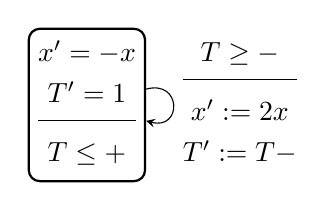
\begin{tikzpicture}
	\node[draw, rectangle, rounded corners,thick] (loc) {
		\begin{tabular}{@{} c @{}}
		$x' = -x$ \\[1mm]
		$T' = 1$ \\[1mm]
		\hline \\[-2mm]
		$T \leq \Tsample + \jitter$
		\end{tabular}};
	%
	\draw[->,>=stealth, loop right,looseness=3] (loc) to node[right] {
		\begin{tabular}{@{} c @{}}
		$T \geq \Tsample - \jitter$ \\[1mm]
		\hline \\[-2mm]
		$x' := 2 x$ \\[1mm]
		$T' := T - \Tsample$
		\end{tabular}} (loc);
\end{tikzpicture}
